% Autogenerated translation of OIA.md by Texpad
% To stop this file being overwritten during the typeset process, please move or remove this header

\documentclass[12pt]{book}
\usepackage{graphicx}
\usepackage{fontspec}
\usepackage[utf8]{inputenc}
\usepackage[a4paper,left=.5in,right=.5in,top=.3in,bottom=0.3in]{geometry}
\setlength\parindent{0pt}
\setlength{\parskip}{\baselineskip}
\setmainfont{Helvetica Neue}
\usepackage{hyperref}
\pagestyle{plain}
\begin{document}

\chapter*{OIA project overview}

\section*{Module 1: Optical immunoassay project}

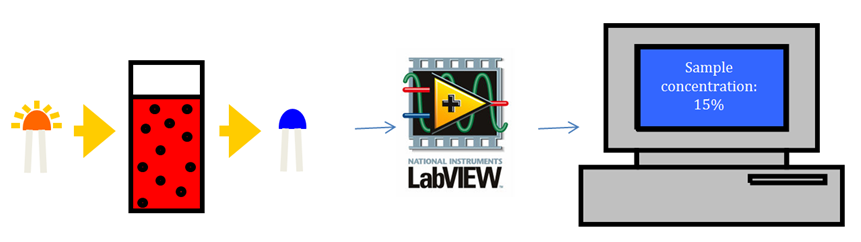
\includegraphics{project_1_OIA/OIA_diagram.png}

\subsection*{Project information}

\begin{itemize}
\item \href{project_1_OIA/project_1_OIA.pdf}{Assignment description and learning objectives}
\item \href{project_1_OIA/OIA_report_rubric.pdf}{Report rubric}
\end{itemize}

\subsection*{Weekly lab exercises}

\begin{itemize}
\item Week 1 (08/22): \href{project_1_OIA/OIA_lab_1.pdf}{Lab protocol} and \href{project_1_OIA/OIA_lab_1_assignment.pdf}{in class assignment}
\item Week 2 (08/29): \href{project_1_OIA/OIA_lab_2.pdf}{Lab protocol} and \href{project_1_OIA/OIA_lab_2_assignment.pdf}{in class assignment}
\item Week 3 (09/12): \href{project_1_OIA/OIA_lab_3.pdf}{Lab protocol} and \href{project_1_OIA/OIA_lab_3_assignment.pdf}{in class assignment}
\item Week 4 (09/19): \href{project_1_OIA/OIA_lab_4.pdf}{Lab protocol} and \href{project_1_OIA/OIA_lab_4_assignment.pdf}{in class assignment}
\item Week 5 (09/26): \textbf{Project demos and report due!}
\end{itemize}

\end{document}
